\chapter{Case Study 2 (Liar's Dice)}
\label{cs2:liars_dice}

In this case study, we introduce Liar's Dice, a dice game utilising hidden information. We introduce partially observable MDPs (known as POMDPs) to represent this hidden information, model a small version of the game using a POMDP, and analyse the susceptibility of Liar's Dice to the snowball effect.

\section{Liar's Dice description}
\label{cs2:liars_dice_description}
Liar's Dice is a dice game for multiple players, where each player must be able to bluff and detect opponent's bluffs in order to win. Liar's Dice takes place over a series of rounds, where each player rolls their dice, keeping the values on the dice hidden from other players. A player then makes a \emph{bid}, which is comprised of a face value on a dice, and the number of dice that show that value. Players then rotate in turn, choosing to either make a higher bid (with either a higher face value, a higher quantity, or both), or challenge the previous bid. If a challenge is made, all dice are revealed. If the bid was correct, the challenging player loses a die. If the bid was incorrect, the bidding player loses a die. The player who lost starts the next round, and play continues until only one player has any remaining dice.

In Liar's Dice, every player starts with the same amount of information, since every player starts with the same number of dice. However, as the game progresses, some players will have more dice than others, changing bidding behaviour, as demonstrated by the following example.

\begin{example}
\label{cs2:hidden_info_example}

Consider the situation presented in Figure \ref{cs2:uneven_information}, where the first player has rolled two 2s while the second player has rolled a 5. The first player can confidently make a bid that there are two 2s, but the second player cannot see enough dice to determine the correctness of this bid. Hence, the second player has three options:

\begin{itemize}

\item if the second player challenges the bid, they will lose a dice, and therefore lose the game;
\item if the second player increases the face value of the bid, then the first player can immediately challenge the bid and win the game, since they know that at most one die cannot have value 2;
\item if the second player increases the quantity of the bid, to bidding that there are three 2s, the first player can challenge and win with probability $\frac{5}{6}$.

\end{itemize}

As a result, the first player is able to use their increased access to information in order to increase their chances of success.

\end{example}

\begin{figure}[h]
    \centering
    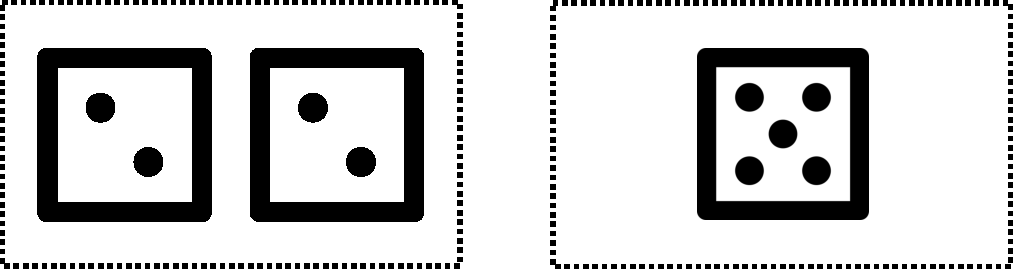
\includegraphics[width=0.7\textwidth]{images/LiarsDice/different_information.pdf}
    \caption{A game of Liar's Dice, where the first player has rolled two 2s while the second player has rolled a 5.}
    \label{cs2:uneven_information}
\end{figure}

This example represents a potential issue with the design of Liar's Dice. Initially we expect that the probability of either player losing a round is even, depending primarily on the strategies the players employ. However, as the game progresses, players with fewer dice are more likely to lose subsequent rounds, making it harder and harder for players to win from behind, a phenomenon known as the \emph{snowball effect} in game design. 

In particular, the snowball effect means that the overall results of games may be decided fairly early on, even if the games are long. This is frustrating for players - the players are still required to play several rounds of a game where the result is already a foregone conclusion. Moreover, with multiple players, this presents an opportunity for one player to be eliminated very early, since the game continues without their involvement.

Our aim when analysing Shut the Box will be to examine to what extent Liar's Dice exhibits the snowball effect, and whether this effect can be mitigated in some way. Firstly, we introduce a variant of MDPs which allows for partial observability, in order to model the hidden information present in Liar's Dice.

\section{Background (1 page)}

A key aspect of Liar's Dice is partial observability, which we now introduce in order to augment our existing MDPs, as described in \cite{norman_verification_2017}.

\begin{definition}
    \label{cs2:def-pomdps}

    A partially observable Markov decision process (or POMDP) is a tuple $\mathcal{P} = (S, \bar{s}, A, \delta, L, \mathcal{O}, obs)$ such that:

    \begin{itemize}
        \item $(S, \bar{s}, A, \delta, L)$ is an MDP, as in Definition \ref{cs1:def_mdps}.
        \item $\mathcal{O}$ is a finite set of \emph{observations}.
        \item $obs : S \rightarrow 2^{\mathcal{O}}$ labels each state with a subset of observations.
        \item For any two states $s, s' \in S$, if $obs(s) = obs(s')$ then the available actions at $s$ and $s'$ must be identical. When this occurs, we say that states $s$ and $s'$ are \emph{observationally equivalent}.
    \end{itemize}
\end{definition}

The last point in this definition indicates how POMDPs can represent hidden information. Rather than being able to directly access every state, decisions can only be made based on observations. For instance, in many card games, some cards may be visible for a particular player, while others are hidden. In order for two states to be observationally equivalent in a model of this game, we only require that the visible cards are the same in both states, while the hidden cards can range across any permutation of valid cards. If a player could view the full state of the game, they would be able to view the value of hidden cards, which would render most of these hidden information games trivial. For Liar's Dice, a player can observe their own dice, the current bid and whether a challenge has been made, but not any opponent's dice.

Since POMDPs are an extension of an MDP, adversaries for POMDPs are defined in terms of adversaries for the corresponding MDP. However, in order to reflect the added constraints that observations provide, we require that adversaries on observationally equivalent paths are equivalent:

\begin{definition}
\label{cs1:pomdp_strats}

For a POMDP $P$, an adversary of $P$ is a function $\sigma$ mapping all finite paths through the POMDP to a discrete probability distribution over the set of actions. In particular, $\sigma$ is also an adversary of the corresponding MDP. Moreover, for paths
\[
\pi = s_0 \xrightarrow{a_0} s_1 \xrightarrow{a_1} \dots s_n \;\;\ \mbox{and} \;\; \pi = s'_0 \xrightarrow{a'_0} s'_1 \xrightarrow{a'_1} \dots s'_n
\]
if $obs(s_i) = obs(s'_i)$ and $a_i = a'_i$ for all $i \in \mathbb{N}$, then $\sigma(\pi) = \sigma(\pi')$. In other words, $\sigma$ makes the same decisions after observationally equivalent paths.

\end{definition}

This definition references a key difference in optimal adversary generation between MDPs and POMDPs. In MDPs, optimal adversaries are deterministic and memoryless, so in particular adversaries map states to actions. This allows for aforementioned methods such as value iteration to be applied, allowing for efficient computation of optimal values and adversaries attaining these optimal values. By contrast, Madani et al. show in \cite{madani_undecidability_2003} that obtaining optimal values and adversaries in POMDPs, both for reachability properties and reward-based properties, is undecideable. We instead focus on approximate solutions, as discussed in the following section.

\subsection{Belief MDPs}

First, we introduce the \emph{belief MDP}. Given a POMDP, we may construct an equivalent MDP, which consists of beliefs of which observationally equivalent state the player is in at any point.

\begin{definition}
    \label{cs2:belief_mdps}

    Given a POMDP $\mathcal{P} = (S, \bar{s}, A, \delta, L, \mathcal{O}, obs)$, as in Definition \ref{cs2:def-pomdps}, the \emph{belief MDP} of $\mathcal{P}$ is given by $\mathcal{B}(\mathcal{P}) = (Dist(S), \delta_{\bar{s}}, A, \delta^\mathcal{B}, L)$. In particular the states of this MDP represent \emph{beliefs} about the state of the player in the corresponding POMDP, and the transition function becomes:

    \begin{equation*}
        \delta^{\mathcal{B}}(b, a)(b') = \sum_{s \in S} b(s) \cdot \left( \sum_{o \in \mathcal{O} \wedge b^{a,o} = b'} \left(  \sum_{s' \in S \wedge obs(s')=o} \delta(s, a)(s') \right) \right)
    \end{equation*}

    In particular, $b^{a, o}$ represents the belief reached after performing action $a$ with observation $o$ in belief $b$, calculated as:

    \begin{equation*}
        b^{a, o}(s') =
        \begin{cases}
            \frac{\displaystyle \mbox{$\sum\nolimits_{s \in S}$} \delta(s, a)(s') \cdot b(s)}{\displaystyle \mbox{$\sum\nolimits_{s \in S}$} b(s) \cdot \left(\mbox{$\sum_{s'' \in S \wedge obs(s'')=o}$} \delta(s,a)(s'')\right)} & obs(s') = 0 \\ 0 & \text{otherwise} \\
        \end{cases}
    \end{equation*}

\end{definition}

We also need to modify how state and transition rewards are calculated for a belief MDP.

\begin{definition}
    \label{cs2:belief_rewards}
    Let $\rho$ be a state reward function and $\iota$ be an action reward function for some POMDP $\mathcal{P}$. For the corresponding belief MDP, we set:

    \begin{align*}
        \rho^{\mathcal{B}}(b) &= \sum_{s \in S} \rho(s) \cdot b(s) \\
        \iota^{\mathcal{B}}(b, a) &= \sum_{s \in S} \iota(s, a) \cdot b(s) \\ 
    \end{align*}

\end{definition}

In particular, this modification of rewards ensures that reachability and reward-based properties coincide between the POMDP and its corresponding belief MDP.

One key remark about this belief MDP is that its state space is now continuous, since the states of the belief MDP represent probability distributions of states in the POMDP. This means that the number of states in the belief MDP is infinite (indeed, uncountably infinite), so the techniques introduced from Section \ref{cs1:prob_reach_mdps} are no longer feasible. Instead, we use a finite set of grid points in order to obtain an upper bound of the property in question, then directly generate a strategy on the POMDP itself to obtain a lower bound. These steps are described in more detail in the following section.

\subsection{Property verification in POMDPs}
\label{cs2:properties_pomdps}

For simplicity, we only describe maximum reachability probabilities - the other cases, including minimum probabilities and expected rewards, are similar.

First, we obtain an upper bound for the property in question. The key idea, as presented by Bertsekas and Yu in \cite{bertsekas_approximate_2006}, is to consider a finite set of states in the belief MDP, known as \emph{representative beliefs}, which form a convex hull of $Dist(S)$. Multiple methods are possible for choosing these representative beliefs, with the simplest method producing a uniform grid $G_M$ as follows:

\begin{equation*}
    G_M = \left\{\frac{1}{M} v \mid v \in \mathbb{N}^{|S|} \wedge \mbox{$\sum_{i=1}^{|S|}$} v_i = M \right\}
\end{equation*}

In particular, we note that the beliefs in $G_M$ are a subset of $\mathbb{Q}_{\geq 0}^{|S|}$, which is countable but still infinite. Hence, this is an approximation of $Dist(S)$, since beliefs containing irrational probabilities can never be included in $G_M$ for any $M$.

The resolution of the grid is denoted by $M$. The number of grid points in $G_M$ is the number of non-negative integer solutions to the equation $v_1 + \dots + v_{|S|} = M$, which is equal to ${M + |S| - 1 \choose M}$. Hence, the grid size is exponential in $M$.

When this grid has been defined, value iteration is applied to the belief MDP, in the same manner as Section \ref{cs1:value_iteration}. However, for beliefs which are not in $G_M$, interpolation is applied, such as via Freudenthal triangulation as discussed further in \cite{lovejoy_computationally_1991}, in order to avoid directly computing values for all beliefs in the belief MDP.

During this process of value iteration, in a very similar manner to Section \ref{cs1:adversary_gen}, an adversary $\sigma^*$ can be obtained, and the DTMC induced under $\sigma^*$ can be solved in order to obtain an approximation for the desired property. However, this adversary is a finite-memory adversary, and as previously discussed this will not always suffice for determining an optimal adversary for a POMDP. As a result, the value obtained under this strategy is a lower bound for the optimal value.

Finally, the resolution of the grid $M$ can be increased in order to yield tighter bounds on the optimal value, with the caveat that, since grid size is exponential on M, care must be taken to ensure these bounds can still be computed in reasonable time.

We have now defined an extension to MDPs which allow us to model games which utilise hidden information. Now, we model and analyse Liar's Dice to show an example of such a game.

\section{Results and analysis}

In this case study, our main aim is to analyse Liar's Dice in order to determine its susceptibility to the snowball effect, as discussed in Section \ref{cs2:liars_dice_description}. We also discuss the implications of POMDPs on model size.

\subsection{State space reduction}

As discussed in Sections \ref{cs2:belief_mdps} and \ref{cs2:properties_pomdps}, verifying properties of POMDPs involves constructing an approximation of the belief MDP, and in particular the size of the grid presented in \ref{cs2:properties_pomdps} increases exponentially with the number of states in the POMDP. Hence, in order to allow for efficient analysis, reducing the number of states in the POMDP is crucial.

For Liar's Dice, the key method employed to reduce model size is to model each \emph{round}, as opposed to each \emph{game}. There are four main reasons why this construction is preferred:

\begin{itemize}
    \item Rounds in Liar's Dice are mostly independent - the main parameters of each game are the number of dice for each player, along with the starting player, which is always the loser of the previous round, or the first player in the first round of the game. Hence, transitioning between rounds is straightforward, since little to no information is maintained between rounds.
    \item As a result of the previous point, some configurations may appear multiple times throughout a game. For instance, suppose each player starts with 3 dice. If player 1 loses the first round while player 2 loses the following two rounds, then player 1 has 2 dice, player 2 has 1 die, and player 2 starts the 4th round. This also occurs when player 2 loses the first and third rounds, while player 1 loses the second round. Hence, we would like to store the results of this round, in order to avoid computing this round on multiple occasions. In essence, this is a form of dynamic programming for model checking.
    \item As an extension of the previous point, some nodes are symmetrical, such as the left and right children of the root node in Figure \ref{cs2:2_dice_game_tree}. This means that separate computation of each of these nodes is unnecessary, so symmetry can be exploited in order to further reduce computation.
    \item If user-defined strategies are employed, then the strategy used by each player can be freely exchanged between rounds. This is especially important for Liar's Dice, since we would expect that a player who has more dice than their opponents would play differently to a player with only one die.
\end{itemize}

\begin{figure}[h]
    \centering
    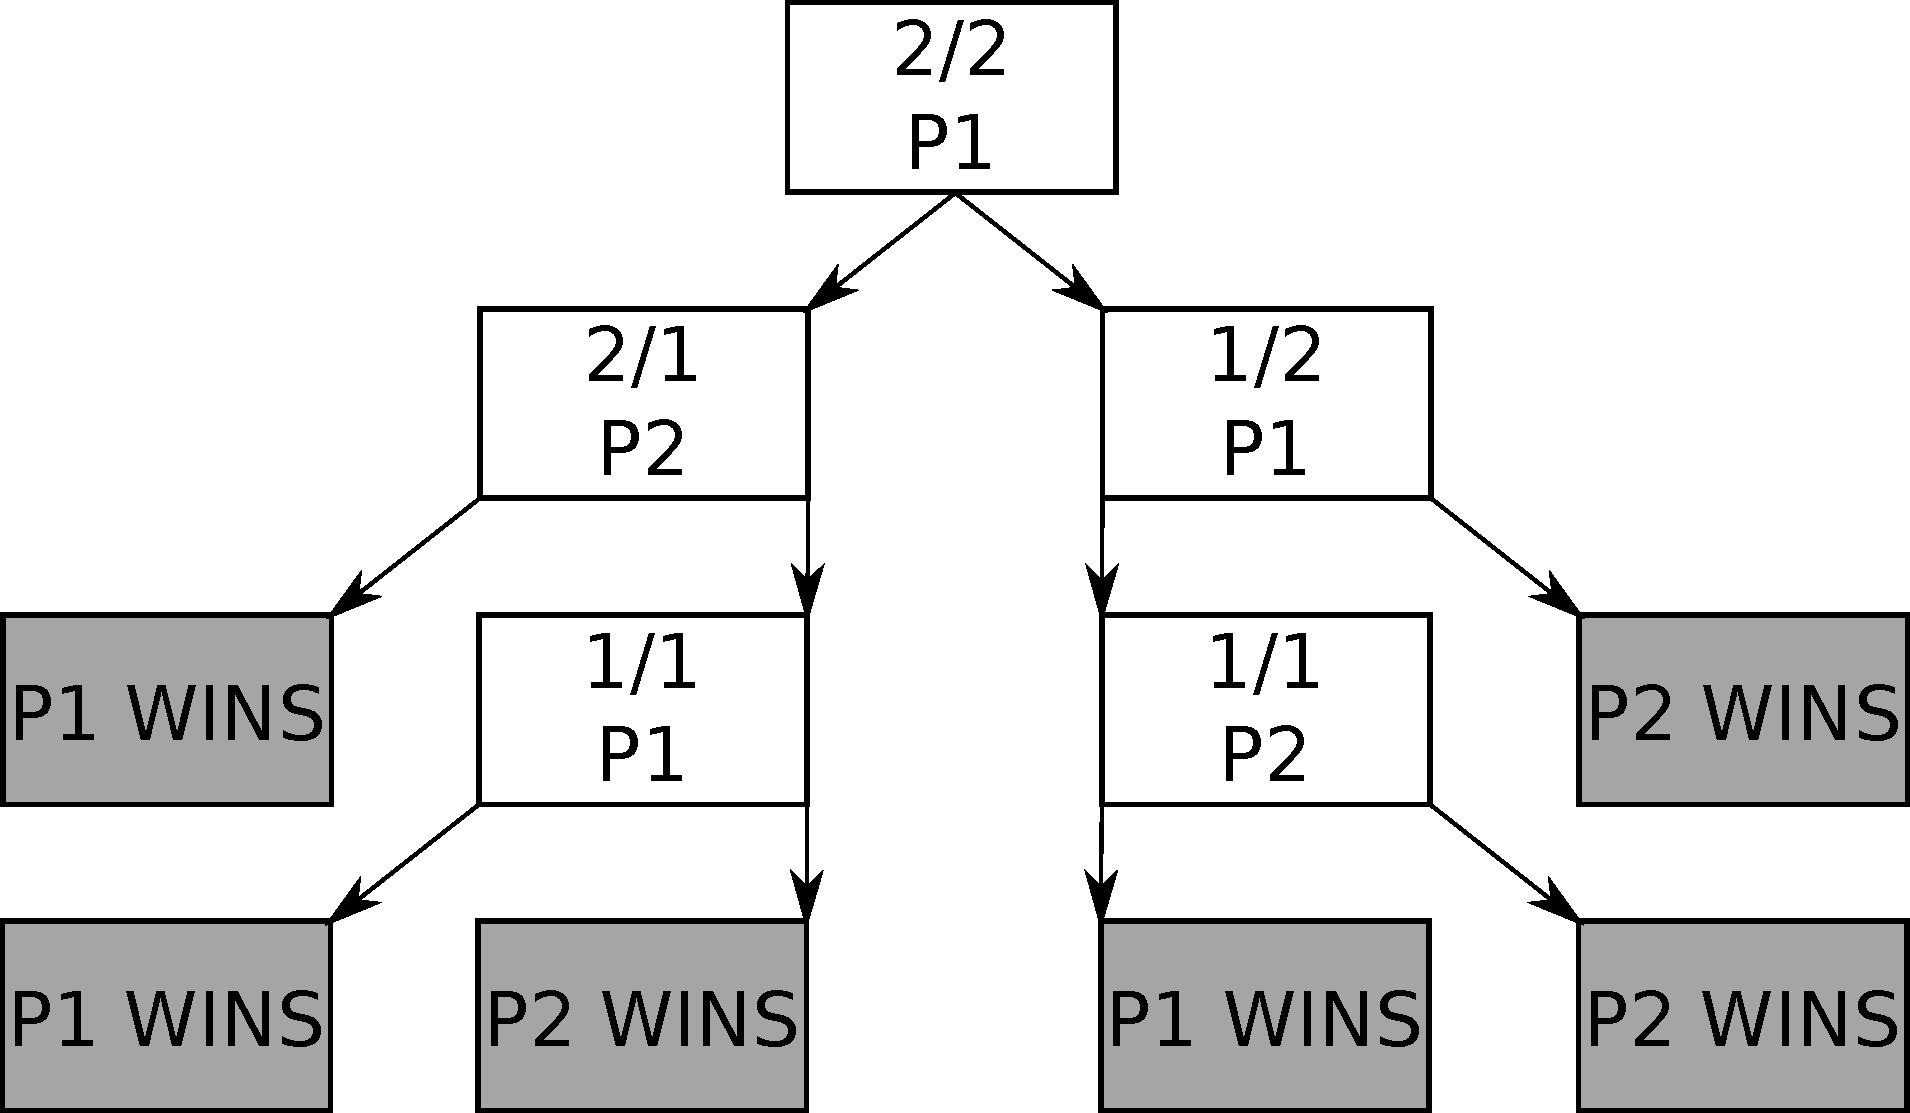
\includegraphics[width=0.7\textwidth]{images/LiarsDice/2_dice_game_tree.pdf}
    \caption{A game tree of Liar's Dice. Each player starts with 2 dice, and each node represents the number of dice player 1 and player 2 have respectively, along with the starting player for that round.}
    \label{cs2:2_dice_game_tree}
\end{figure}

This construction allows us to define a \emph{game tree}, as in Figure \ref{cs2:2_dice_game_tree}, where each node represents one round of the game. This construction allows for simpler computation of the probability of a player winning a game. Rather than check a property for one large model, we check the win rate for each smaller model, then traverse the tree, obtaining a weighted sum based on the probability of winning each round.

Another key implication of using game trees is that sub games can be considered very easily. For instance, in the game presented in Figure \ref{cs2:2_dice_game_tree}, a handicap can easily be considered, since the right child of the root node represents handicapping player 1 by removing one of their dice at the start of the game.

\subsection{Model constraints}

Due to the requirement to reduce model size, several assumptions and limitations were imposed on the model. In particular, rather than being able to make any bids, players are assumed to only either increase the face value by 1 or increase then quantity of the bid by 1. This limits the number of possible actions per bid, since there are now only two types of bids, plus the option of challenging the other player. Another key limitation is that we only consider variants of Liar's Dice with two players, and at most 2 dice per player.

\subsection{Pre-defined strategies}

As with our first case study, we define some initial strategies in order to make comparisons to the optimal strategy. In Liar's Dice, there are three main types of decision to make. Firstly, the initial bid is important, since an aggressive opponent could start with a high bid and force an opponent to make an early decision about bluffing, without having enough time to gather information and form beliefs. Secondly, the decision to challenge is important - an overly aggressive strategy will lose frequently due to bidding on correct bids, while an overly conservative strategy will eventually make a bid that the opposing player can confidently challenge. Finally, the type of bid is also important - in general we expect increasing the quantity of a bid to be riskier than increasing the face value of a bid, since increasing the quantity provides more information for players to potentially challenge the bid.

We now introduce two main types of player, exemplifying the different possibilities for each of these types of decisions. The \emph{risky player} makes a random bid at the start of the game, even where this bid may be initially incorrect. When bidding, they always increase the quantity of the bid where possible before increasing face value, and they always challenge when the sum of the face value and quantity is at least half the maximum possible sum. The \emph{safe player} makes a random bid at the start of the game, but only a bid which is guaranteed to appear in their hand. When bidding, they always prioritise increasing the face value of the bid rather than the quantity, and always challenge when the sum of the face value and quantity is at least 75\% of the maximum possible sum.

It is important to note that these strategies are deliberately very simple, and unlikely to be effective. This is by design - here we are more interested in comparing various rounds of the game, as opposed to different strategies. These strategies are designed to represent the extremes of possible behaviour in Liar's Dice, in order to provide comparisons for optimal strategies.



\section{Evaluation (2 pages)}

Again, use model checking results to answer questions about Liar's Dice. Discuss potential limitations of analysis that arise from using POMDPs.

